\documentclass[10pt,conference,letterpaper]{IEEEtran}
\usepackage{times,amsmath,epsfig}
%
\title{XCPU2 Process Management System}
%
\author{%
{Latchesar Ionkov{\small $~^{\#1}$}, Eric Van Hensbergen{\small $~^{*2}$} }%
\vspace{1.6mm}\\
\fontsize{10}{10}\selectfont\itshape
$^{\#}$\,Los Alamos National Laboratory\\
Los Alamos, NM 87545, USA\\
\fontsize{9}{9}\selectfont\ttfamily\upshape
$^{1}$\,lionkov@lanl.gov\\
\vspace{1.2mm}\\
\fontsize{10}{10}\selectfont\rmfamily\itshape
$^{*}$\,IBM Austin Research Laboratory\\
Address Including Country Name\\
\fontsize{9}{9}\selectfont\ttfamily\upshape
$^{2}$\,bergevan@us.ibm.com
}
%

\begin{document}
\maketitle
%
\begin{abstract}

Xcpu2 is a new process management system that allows the users to
specify custom filesystem for a running job. Most cluster management
systems enforce single software distribution running on all nodes.
Xcpu2 allows programs running on the cluster to work in environment
identical to the user's desktop, using the same versions of the
libararies and tools the user installed locally, and accessing the
configuration file in the same places they are located on the desktop.

Xcpu2 builds on our earlier work with the Xcpu system. Like Xcpu,
Xcpu2's process management interface is represented as a set of files
exported by a 9P file server. It suppports heterogeneous clusters and
multiple head nodes. Unlike Xcpu, it uses pull instead of push model.

In this paper we describe the Xcpu2 clustering model, its operation
and how the per-job filesystem configuration can be used to slve some
of the common problems when running a cluster.

\end{abstract}

\section{Introduction}

Xcpu2 is a remote process management system that represents execution and
control services as a set of files in the file system. The file system can
be mounted over the network. By manipulating the exported files, the
client-side tools create an execution environment, execute and control the
process remotely.

A typical HPC cluster has a large number of compute nodes and a single
control/head node. It uses a parallel file system, that run on separate set
of nodes, usually physically separated from the rest of the cluster. The
control node is used to run the software that monitors the cluster health,
the job scheduler that is used for scheduling and executing jobs as well as
the compute node booting service. In most cases the compute nodes don't have
local disks, or if they do, they are only used for scratch space and don't
have an operating system installed. The compute nodes receive the operating
system kernel and disk image over the network and store their file system in
the node's RAM. In order to save memory and improve the booting time, the
system images are tens-to-hundreds of megabytes large and contain only the
most commonly used libraries and tools. Most of the cluster installations
support a single sistem image that is running on all compute nodes. Adding
new software, or upgraiding the existing one is a complex task that requires
coordingation between the cluster support group and all teams that use the
cluster. Upgrading a library required to run a new scientific code can take
weeks and months. The overhead and the time required for the coordination
makes it hard for groups to share clusters.

In typical cluster environments the application developers are forced to use
the same software image on their desktop, or have a dedicated development
server to ensure that the application will execute correctly on the cluster.

There are attempts to make the cluster environment more flexible and allow
the users to pick from a limited set of system images. The most common
approach is to use hypervisors on the compute nodes and create a cluster of
virtual machines that use the preferred system image. Another approach
requires rebooting the nodes assigned to a job with the requested image.
Both solutions cause some performance degradation.

Ideally the cluster user would like, when running on the cluster, his job to
have the same environment it has when running on his desktop or development
server. Thay way he can use his favorite tools and libraries without
worrying about compatibility with the system image.

Xcpu2 allows the user to configure the view of the filesystem that will be
used when the job is run. It uses Linux support of private namespaces and
provides each job with its own filesystem view. Xcpu2 allows parts of the
original filesystem to be ``bound'' to other locations, remote filesystems
to be mounted. In the Xcpu2 cluster model, the control node is used to
allocate nodes for a job, but the job control can be performed from any
other computer, including the user's desktop. In addition to controlling the
running job, the client-side tools export the filesystem of the controlling
computer, so it can be mounted and used by the compute nodes assigned for
the job. By using a filesystem configuration, all compute nodes can be
configured to have file system that is identical to the user desktop.

When a single application is run on multiple nodes, it is very likely that
the nodes will access the same files. All nodes will run the same
executable, use the same shared libraries and read the same configuration
files. Caching mechanisms that use that fact would have much better
hit-to-miss ratio than the general-purpose ones. Xcpu2 currently provides a
simple read-only hierarchical caching in order to improve the performance.

\section{Related Work}

There are many process and resource management systems for clusters. In this
section we are going to describe the ones that influenced the development of
Xcpu2, or are trying to provide the user with similar environment.

The Beowulf Distributed Process Space (Bproc)~\cite{bproc} is a set of
Linux kernel modifications and user-space daemons that allows a user on the head
node to see the processes on all cluster nodes as local processes and
manipulate them with the standard Unix tools. Remote processes can be
examined, killed or debugged from the head node without any modifications of
the binary. The process view provided by Bproc is asymmetric, tools running
on the compute nodes still see only the local processes. That asymmetry as
well as the high cost of maintaining a Linux kernel patch outside of the
standard kernel distribution lead to exploring other more convenient solutions.

Xcpu~\cite{ron-xcpu} is a process management system developed at LANL to
replace Bproc. The Xcpu system consists of a daemon (xcpufs) that runs on
each compute node, and a set of tools running on the head node. Xcpufs
creates a synthetic filesystem that can be mounted on Linux and Plan9, or
accessed via user space tools. Manipulation of the synthetic files allows
retrieving the state of the node, list of the processes or jobs running on
it and their running environment. The file interface also allows creation,
control and destruction of jobs. Xcpu implements a push model: the
executable for the job is tranfrerred from the head node to all compute
nodes explicitly. Xcpu can push multiple files per job, so in addition to
the binary, it can also transfer all shared libraries it depends on,
configuration and data files required for the job's operation. On ELF
systems, like Linux and Solaris, Xcpu can automatically detect and transfer
all shared libraries an executable depends on. This feature is very useful
on clusters with diskless compute nodes that are only using minimal OS
images. Xcpu supports heterogeneous clusters automatically distributing the
appropriate binary for each architecture. The xcpufs file hierarchy and and
the operations performed on each file are described in details in
\cite{lucho-xcpu}.

Xcpu's state is distributed across all compute nodes, each node keeping its
own state. If a control node crashes the rest of the cluster doesn't need to
be restarted, or any jobs cancelled. All of the jobs can continue running
until the head node is rebooted. Once it is up, it collects the job
information and is in normal operation. Using file system interface also
allows more than one server to mount and control the compute nodes. That
feature allows configurations with hot-spare head nodes.

To improve the job startup stime for large jobs, Xcpu implements a
tree-spawn mechanism (Figure~\ref{fig:xcpu-tspawn}). The nodes assigned for
a job are organized in a tree, with the head node in the root, each node
having no more than adjustable number of children. The head node establishes
the process environment and tranferes the required file to the nodes on the
first level of the tree. It then instructs them to \textsl{clone} their
state to their children. Once all nodes have their state set up, the head
node destroys the tree and starts the job execution.

\begin{figure}[h]
\begin{center}
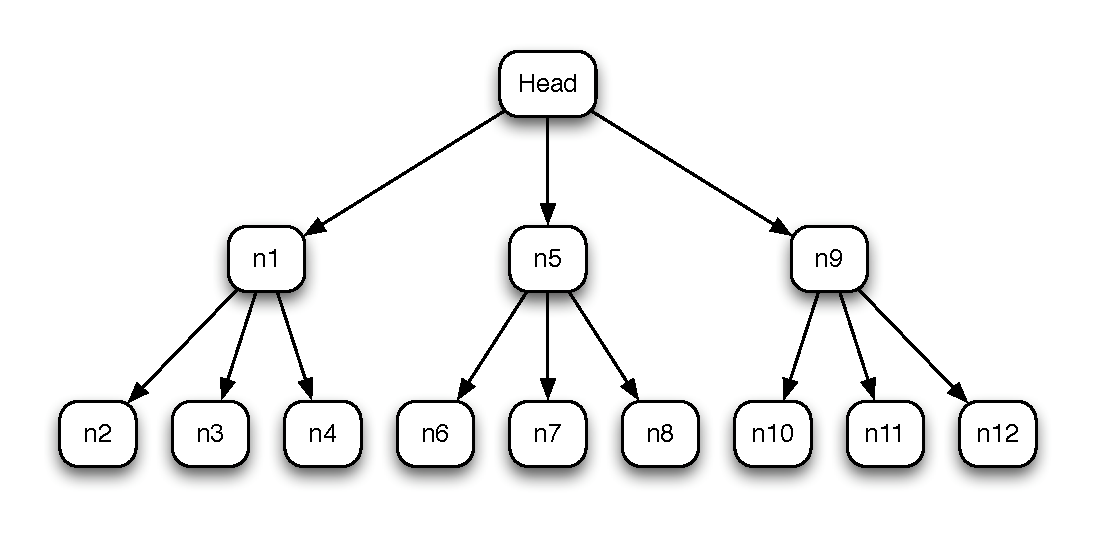
\includegraphics[width=3in, keepaspectratio]{xcpu-tspawn.eps}
\end{center}
\caption{Xcpu tree-spawn applied to a 12-node job, with 3 children per node.}
\label{fig:xcpu-tspawn}
\end{figure}

Xcpu uses the 9P resource sharing protocol. Originally developed for Plan9,
9P is currently supported by the standard Linux kernel. 9P was chosen
because of its simplicity and architecture independence.

Xcpu uses the standard Unix file permissions to ensure that the users only
start jobs to the nodes assigned to them. Xcpufs maintains a list of users
and groups. The ownership of the synthetic files and their read/write
permissions control what operations each user can perform onthe node. In
addition to the user names and IDs, xcpufs stores user's public key that is
used to ensure that the connection is established by the appropriate user.
The authentication scheme is similar to the one used in SSH2~\cite{rfc4252}.

Xcpu borrows some ideas from Plan9's cpu~\cite{plan9-cpu} command. In Plan9
most of the OS and system services are represented as file trees. Operations
on devices and services are performed by normal read and write operations.
In Unix, most of these operations are performed using ioctl's, which by
their nature cannot be performed when the file is mounted on a remote
machine. In Plan9 all devices can be mounted and controlled remotely. The
cpu command uses this feature to reproduce on a remote server exactly the
same filesystem that the user has on his local machine. Because everything
is represented as files, a program running on a remote server that tries to
play a sound, will access the files that represent that are ``connected'' to
the user's local sound card. Using a simple resource sharing protocol and
the ``everything is a file'' concept, Plan9 solves many of the problems that
are being solved one piece at a time in Unix. The cpu command allows the
user to login to a remote server while seeing exactly the same file
namespace that was present on the local machine. The user experience when
using it is like ``importing'' the remote server CPUs and RAM to the local
machine -- everything else in his environment remains identical.

Xcpu2 tries to bring cpu's user experience to the cluster environment and
Linux. It changes some important Xcpu concepts. Instead of pushing the job
executable and supporting files explictly, Xcpu2 exports the file system
from the user's machine to all nodes assigned for the job. Using Linux
private namespaces, Xcpu2 creates private view of the filesystem for each
job running on a node. Xcpu2 allows that view to be configured depending on
the job and the cluster requirements. One of the commonly used file
namespaces is mimicing the cpu command behavior (as close as possible on
Linux) providing a view identical to the one on the user's machine.

TODO: mention systems that use VMs or reboot the nodes with specified images.

\section{XCPU2 Operation}

\subsection{Computer roles}

Xcpu2 recognizes three types (Figure~\ref{fig:xcpu2-nodes}) of computers
that participate in the job execution. The control node runs the tools
responsible for the cluster maintainance -- monitoring, resource management
and job scheduling. The compute nodes are assigned temporarily to a job and
run the user applications. Once the resource manager assigned a number of
compute nodes to a job, they are handed over to the job control machine,
which is respobsible of preparing them for the job, running it, monitoring
and controlling its progress. Once the job finishes, the job control machine
hands the nodes back to the resource manager so they can be used by another
job. In some cases the control node is also used as a job control node.
In addition to that, Xcpu2 allows the user desktop, or any other computer to
server that role.

\begin{figure}[h]
\begin{center}
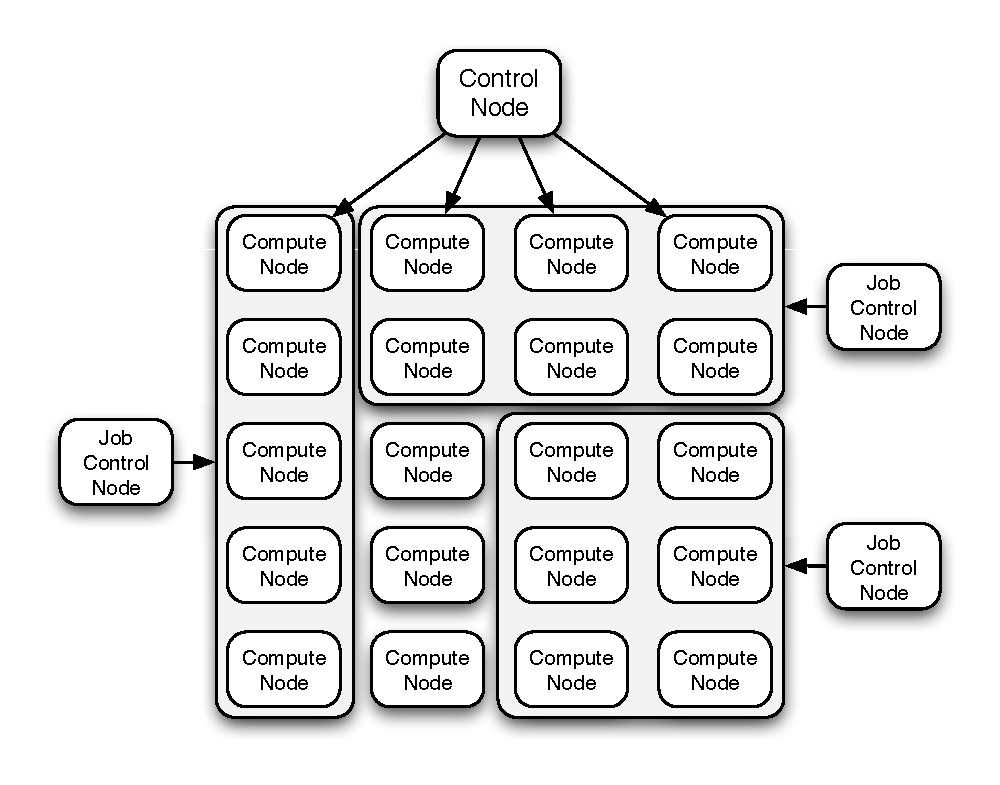
\includegraphics[width=3in, keepaspectratio]{xcpu2-nodes.eps}
\end{center}
\caption{Xcpu2 computer roles}
\label{fig:xcpu2-nodes}
\end{figure}

\subsection{Compute node daemon}

Xcpufs is the xcpu2 daemon that is running on each compute node. It exports
its interface as a file tree. Xcpufs maintains a list of users that can
attach to the interface and perform process management operations remotely.
Xcpufs is implemented as a user space 9P file server and can be accessed
over the network using any 9P client software.

\subsubsection{Xcpufs authentication}

Unlike other network file protocols, 9P requires each user to authenticate
to the server explicitly. Before an user can perform any operations, it
needs to authenticate itself to xcpufs. The daemon allows two authentication
mechanisms. The first one is similar to the challenge-response
authentication used in SSH2. Xcpufs sends a challenge string, the client
signes it with the user's private key, and the daemon verifies the signature
using the user's public key. When the user is already authenticated, he can
read a \textsl{passkey} from the \texttt{passkey} file. The passkey can be
stored or transported to another server and used later to authenticate as
the same user. Each passkey can be used only once.

\subsubsection{Xcpufs sessions}

Xcpu2 allows more than one job running on a compute node at the same time. A
job is comprised of many xcpufs \textsl{sessions} running on multiple
nodes. Each session defines a single program that is run on a single node as
a part of the job. The session defines program's environment, its arguments,
the filesystem view as well as the name of the program to run. Once the
program is running, the user can send data to its standard input, read its
standard output or error streams, or send signals. When the program
terminates, the user can read program's exit code.

Each session on the node is represented as a directory that contains the
files used to control it. Table~\ref{tbl:xcpu2-session} lists the session
files and their purpose.

\begin{table}[ht]
\begin{center}
\begin{tabular}{lp{2.4in}}
    Name & Description\\
    \hline
    \ttfamily ctl & Session control file\\
    \ttfamily argv & Program arguments\\
    \ttfamily env & Program environment variables\\
    \ttfamily stdin & Standard input stream\\
    \ttfamily stdout & Standard output stream\\
    \ttfamily stderr & Standard error stream\\
    \ttfamily wait & Exit code. Reading blocks until program termination\\
    \ttfamily id & Job ID (set by the client)\\
    \ttfamily ns & Session namespace\\
\end{tabular}
\caption{Session files}
\label{tbl:xcpu2-session}
\end{center}
\end{table}

A new session is created by opening the top-level \texttt{clone} file. The
open operation creates a new session and its corresponding directory.
Reading from the opened \texttt{clone} file returns the session ID, which is
the same as the session directory name. The session directory remains
accessible as long as there is at least one file in it that is open, or
until the program associated with the session is running. Once the program
terminates and all session files are closed, xcpufs destroys the session and
releases all resources it used.

\begin{table}[ht]
\begin{center}
\begin{tabular}{lp{1.9in}}
    Command & Description\\
    \hline
    exec \textsl{filename} & Execute the program. Can be used only once\\
    wipe & Kill the program if running and destroy the session\\
    signal \textsl{signame} & Send signal to the running program\\
    close std{\ldots} & Close the specified standard stream\\
    redirect std{\ldots} \textsl{file} & Redirect the standard stream from/to the file\\
    id \textsl{ID} & Set session job ID\\
\end{tabular}
\caption{Session commands}
\label{tbl:xcpu2-sctl}
\end{center}
\end{table}

Session's \texttt{ctl} file is used to control the session state. By writing
commands, the user can change its state -- start the program execution, send
signals to the program main process, close or redirect the program standard
streams. A command starts with the command name, followed by a number of
arguments separated by the space character, and ends with a new-line
character. Table~\ref{tbl:xcpu2-sctl} shows the list of session commands
supported by xcpufs.

In order to provide support for multiple head nodes, xcpufs ensures that all
readers from \texttt{stdout} and \texttt{stderr} receive all the data. 

\begin{table}[ht]
\begin{center}
\begin{tabular}{lp{1.9in}}
    Command & Description\\
    \hline
    unshare & Create private file namespace for the session\\
    mount \textsl{dev} \textsl{dir} \textsl{type} \textsl{options} & Mount a filesystem\\
    bind \textsl{olddir} \textsl{newdir} & Bind a subtree from the filesystem to another place \\
    import \textsl{addr} \textsl{dir} & Mount a 9P filesystem\\
    cd \textsl{dir} & Change the current directory\\
    chroot \textsl{dir} & Make \textsl{dir} the root of the filesystem\\
    cache \textsl{addr} & Cache the content of the 9P filesystem locally\\
\end{tabular}
\caption{Namespace commands}
\label{tbl:xcpu2-ns}
\end{center}
\end{table}

The \texttt{ns} file contains a list of instructions on how to build the
session's filesystem namespace before running the program. Xcpufs allows the
session to create its private namespace by using the \textsl{unshare}
command. Once it is specified, all changes to the filesystem (mounts and
binds) are private to the processes that belong to the session, and are not
visible to the rest of the processes running on the node. The namespace file
can contain references to environment variables defined for the session. The
references are replaced with the environment values before the namespace
commands are executed. Table~\ref{tbl:xcpu2-ns} shows all commands that can
be used for the namespace definition. The default session namespace is
defined as:

\begin{verbatim}
  unshare
  import $XCPUTSADDR /mnt/term
  bind /mnt/term/$XCPUARCHDIR /mnt/sandbox
  bind /mnt/term/home /mnt/sandbox/home
  bind /dev /mnt/sandbox/dev
  bind /proc /mnt/sandbox/proc
  bind /sys /mnt/sandbox/sys
  chroot /mnt/sandbox
\end{verbatim}

After creating the private namespace, xcpufs mounts the filesystem exported
by the job control node (contained in the XCPUTSADDR variable), binds the
directory that contains the files for the compute node architecture, binds
the local \texttt{/dev}, \texttt{/proc} and \texttt{/sys} directories at the
appropriate places and makes \texttt{/mnt/sandbox} the root directory of the
namespace. This in effect hides the node's local filesystem from the
program, providing the same filesystem view that it would have if running on
the job control node.

\subsubsection{Top-level files}

The synthetic files on the top level of the xcpufs file tree are used for
operations common to all sessions. Table~\ref{tbl:xcpu2-top} lists their
names and description.

\begin{table}[ht]
\begin{center}
\begin{tabular}{lp{2.4in}}
    Name & Description\\
    \hline
    \ttfamily clone & Create new session\\
    \ttfamily ctl & Node control file\\
    \ttfamily arch & Node's OS and CPU architecture\\
    \ttfamily env & Default session environment\\
    \ttfamily procs & Process list\\
    \ttfamily state & State of the node (set by the client)\\
    \ttfamily passkey & Generate a new passkey for authentication\\
    \ttfamily pwent & List of users\\
    \ttfamily grent & List of groups\\
    \ttfamily ns & Default session namespace\\
\end{tabular}
\caption{Top-level files}
\label{tbl:xcpu2-top}
\end{center}
\end{table}

The \texttt{env} and \texttt{ns} files allow the cluster administrator to
set the default values for all sessions created on the node. When a new
session is created, the initial values of its environment and namespace are
copied from the top-level files. The \texttt{procs} file contains a list of
all processes running on the compute node. The list is represented in
S-expression with first line defining the entries that are returned for each
process. The top-level \texttt{ctl} file accepts commands in the same format
as the session \texttt{ctl} file.

User and group management is performed by using \textsl{user-add},
\textsl{user-del}, \textsl{group-add}, \textsl{group-del},
\textsl{user-add-group} and \textsl{user-del-group} commands. Each user
group has a name, group ID and a list of members. The users have name, ID,
default group and a public key that is used to authenticate them. Xcpufs
defines a special group and user ``xcpu-admin'' with ID 65530. Initially all
xcpufs files are owned by xcpu-admin, so that is the only user that can add
other users. The admin can change the ownership and permission of any file 
using chown and chmod commands. If an user can write to the \texttt{ctl}
file he can add or delete users, kill processes etc. If an user is granted
permission to read from the \texttt{clone} file, he can create new sessions
and run programs on the node.


\subsubsection{Examples on using standard Unix tools to perform xcpufs
operations}

Assuming that the xcpufs filesystem is mounted on /mnt/xcpu, the user can:

Add a new user:

\begin{verbatim}
  echo user-add glenda 500 mammals \
    `ssh-rsa AAA...Sw== glenda@lanl.gov' \
     > /mnt/xcpu/ctl
\end{verbatim}

Kill process with PID 432 on the node:

\begin{verbatim}
  echo kill 432 > /mnt/xcpu/ctl
\end{verbatim}

Create a new session and set the program arguments:

\begin{verbatim}
  tail /mnt/xcpu/clone &
  12
  echo foo bar then > /mnt/xcpu/12/argv
\end{verbatim}

\subsection{Job Control Tools}

\subsection{Cache implementation}

\section{Case Studies}

\section{Performance}

\section{Future work}

\bibliographystyle{IEEEtran}

\bibliography{xcpu2}

\end{document}
